Der Franck-Hertz-Versuch zählt zu einem der ersten Experimente, welches die
Quantennatur der Elektronenhülle eines Atoms bestätigt. Es bestätigte zudem die
Bohr'schen Postulate, die aufgestellt wurden, um Widersprüche zwischen der
Maxwellschen Elektrodynamik und den Ergebnissen aus der Atomspektroskopie
aufzulösen.

Bei dem Franck-Hertz-Versuch handelt es sich um ein Elektronenstoßexperiment,
bei dem Atome mit Elektronen mit geeigneter Energie beschossen werden. Der
Energieverlust der Elektronen dient hierbei als Informationsquelle. Bei diesem
Experiment wechselwirken möglichst monoenergetische Elektronen mit Hg-Dampf
was sowohl elastische, als auch unelastische Stöße zur Folge hat. Die vom
Quecksilber aufgenommene Energie wird hierbei mit der Energiedifferenz der
Elektronen vor und nach dem Stoß berechnet. Diese Energie wird beim unelastischen
Stoß dazu verwendet das Hg-Atom aus seinem Grundzustand $_E0$ in den ersten angeregten
Zustand $E_1$ zu heben. Es gilt somit:
\begin{equation}
  \frac{\su{m_0\cdot v_{vor}^2}}{2}-\frac{\su{m_0\cdot v_{nach}^2}}{2} = E_1-E_0
\end{equation}

In einem evakuierten Gefäß verdampft ein Tropfen Quecksilber, bis sich ein
Sättigungsdruck $p_sat$ einstellt, der abhängig von der Temperatur $T$ ist. Die
Dampfdichte lässt sich somit über die Temperatur steuern.
In einem Glaskolben befindet sich ein Draht, welcher bis zur Rotglut erhitzt
wird. Durch den Glühelektrischen Effekt treten Elektronen in großer Zahl aus und
umgeben den Draht wie eine Wolke. An der Elektrode gegenüber dem Glühdraht wird
eine positive Gleichspannung $U_\su{B}$ angelegt. Die kinetische Energie der
Elektronen nach dem durchlaufen dieser Strecke beträgt
\begin{equation}
  \frac{\su{m_0\cdot v_{vor}^2}}{2}.
  \label{Ekin}
\end{equation}
Nach dieser Elektrode befindet sich eine weitere Elektrode an der ein
Auffängerstrom $I_\su{A}$ und eine geringere Gegenspannung $U_\su{A}$ angelegt.
Es gelangen jedoch nur Elekronen zu dieser Auffängerelektrode, deren
Geschwindigkeitskomponente $v_\su{z}$ die Ungleichung
\begin{equation}
  \frac{\su{m_0}}{2}v_\su{z}^2 \geq e_0U_\su{A}
\end{equation}
erfüllt. Erfüllt ein Elektron diese Ungleichung nicht, kehrt es zur
Beschleunigerelektrode zurück. Die Hg-Atome die sich nun im Beschleunigungsraum
aufhalten stoßen mit Elektronen zusammen. Hierbei werden 2 Fälle unterschieden.
Ist die Elektronenenergie nicht allzu groß, treten elastische Stöße auf. Die
Energie, die das Elektron an das Hg-Atom abgibt ist hierbei vernachlässigbar
gering. im Zentralen Stoß beträgt diese
\begin{equation}
  \Delta E = \frac{\su{4m_0M}}{\su{(m_0+M)^2}}E\approx 1.1\,\cdot10^{-5}E
\end{equation}
da das Massenverhältnis $\su{m_0/M}$ von Elektron und Hg-Atom etwa
$1/1836\cdot201$ beträgt. Die Richtungsänderung die das Elektron erfährt sind
jedoch beträchtlich.
Erreicht die Elektronenenergie einen Wert der größer oder gleich der
Energiedifferenz zwischen dem Grundzustand und dem ersten angeregtem Zustand,
kann das Elektron das Quecksilberatom anregen. Hierbei überträgt das Elektron
genau den Energiebetrag $E_1-E_0$ auf die Elektronenhülle des Hg-Atoms.
Das Hg-Atom geht dann mit einer Relaxationszeit in einer Größenordnung von
$10^{-8}\sek$ in den Grundzustand zurück. Hierbei wird ein Lichtquant mit der
Energie
\begin{equation}
  \su{h}\nu =E_1-E_0
\end{equation}
emittiert. Um festzustellen, wann das Hg-Atom angeregt wird, wird der
Auffängerstrom $I_\su{A}$ in Abhängigkeit der Berschleunigerspannung $U_\su{B}$
beobachtet. Der Elektronenstrom wächst an, wenn die Beschleunigerspannung die
Auffängerspannung übersteigt.

Wenn die Elektronenenergie den Wert $E_1-E_0$ erreicht oder überschreitet, treten
unelastische Stöße auf, bei denen die Elektronen praktisch ihre gesamte Energie
abgeben und somit nicht mehr in der Lage sind gegen das Bremsfeld anzulaufen.
Somit muss der Auffängerstrom stark absinken.
Wenn die Beschleunigerspannung $U_\su{B}$ weiter gesteigert wird, können die
Elektronen wieder Energie aufnehmen, da die Stoßzone nun ein Stück vor der
Beschleunigerelektrode liegt.
Der Auffängerstrom steigt nun wieder an, bis die Elektronen die Energie $E_1-E_0$
erreicht haben und in der Lage sind einen zweiten unelastischen Stoß anzuregen.
Dieser Vorgang lässt sich bei weiterer Steigerung von $U_\su{B}$ noch einige
Male wiederholen. Der Verlauf des Auffängerstroms in Abhängigkeit zur
Beschleunigungsspannung ist in der unten stehenden Abbildung \ref{fig:kurve} zu
sehen.
\begin{figure}
  \centering
  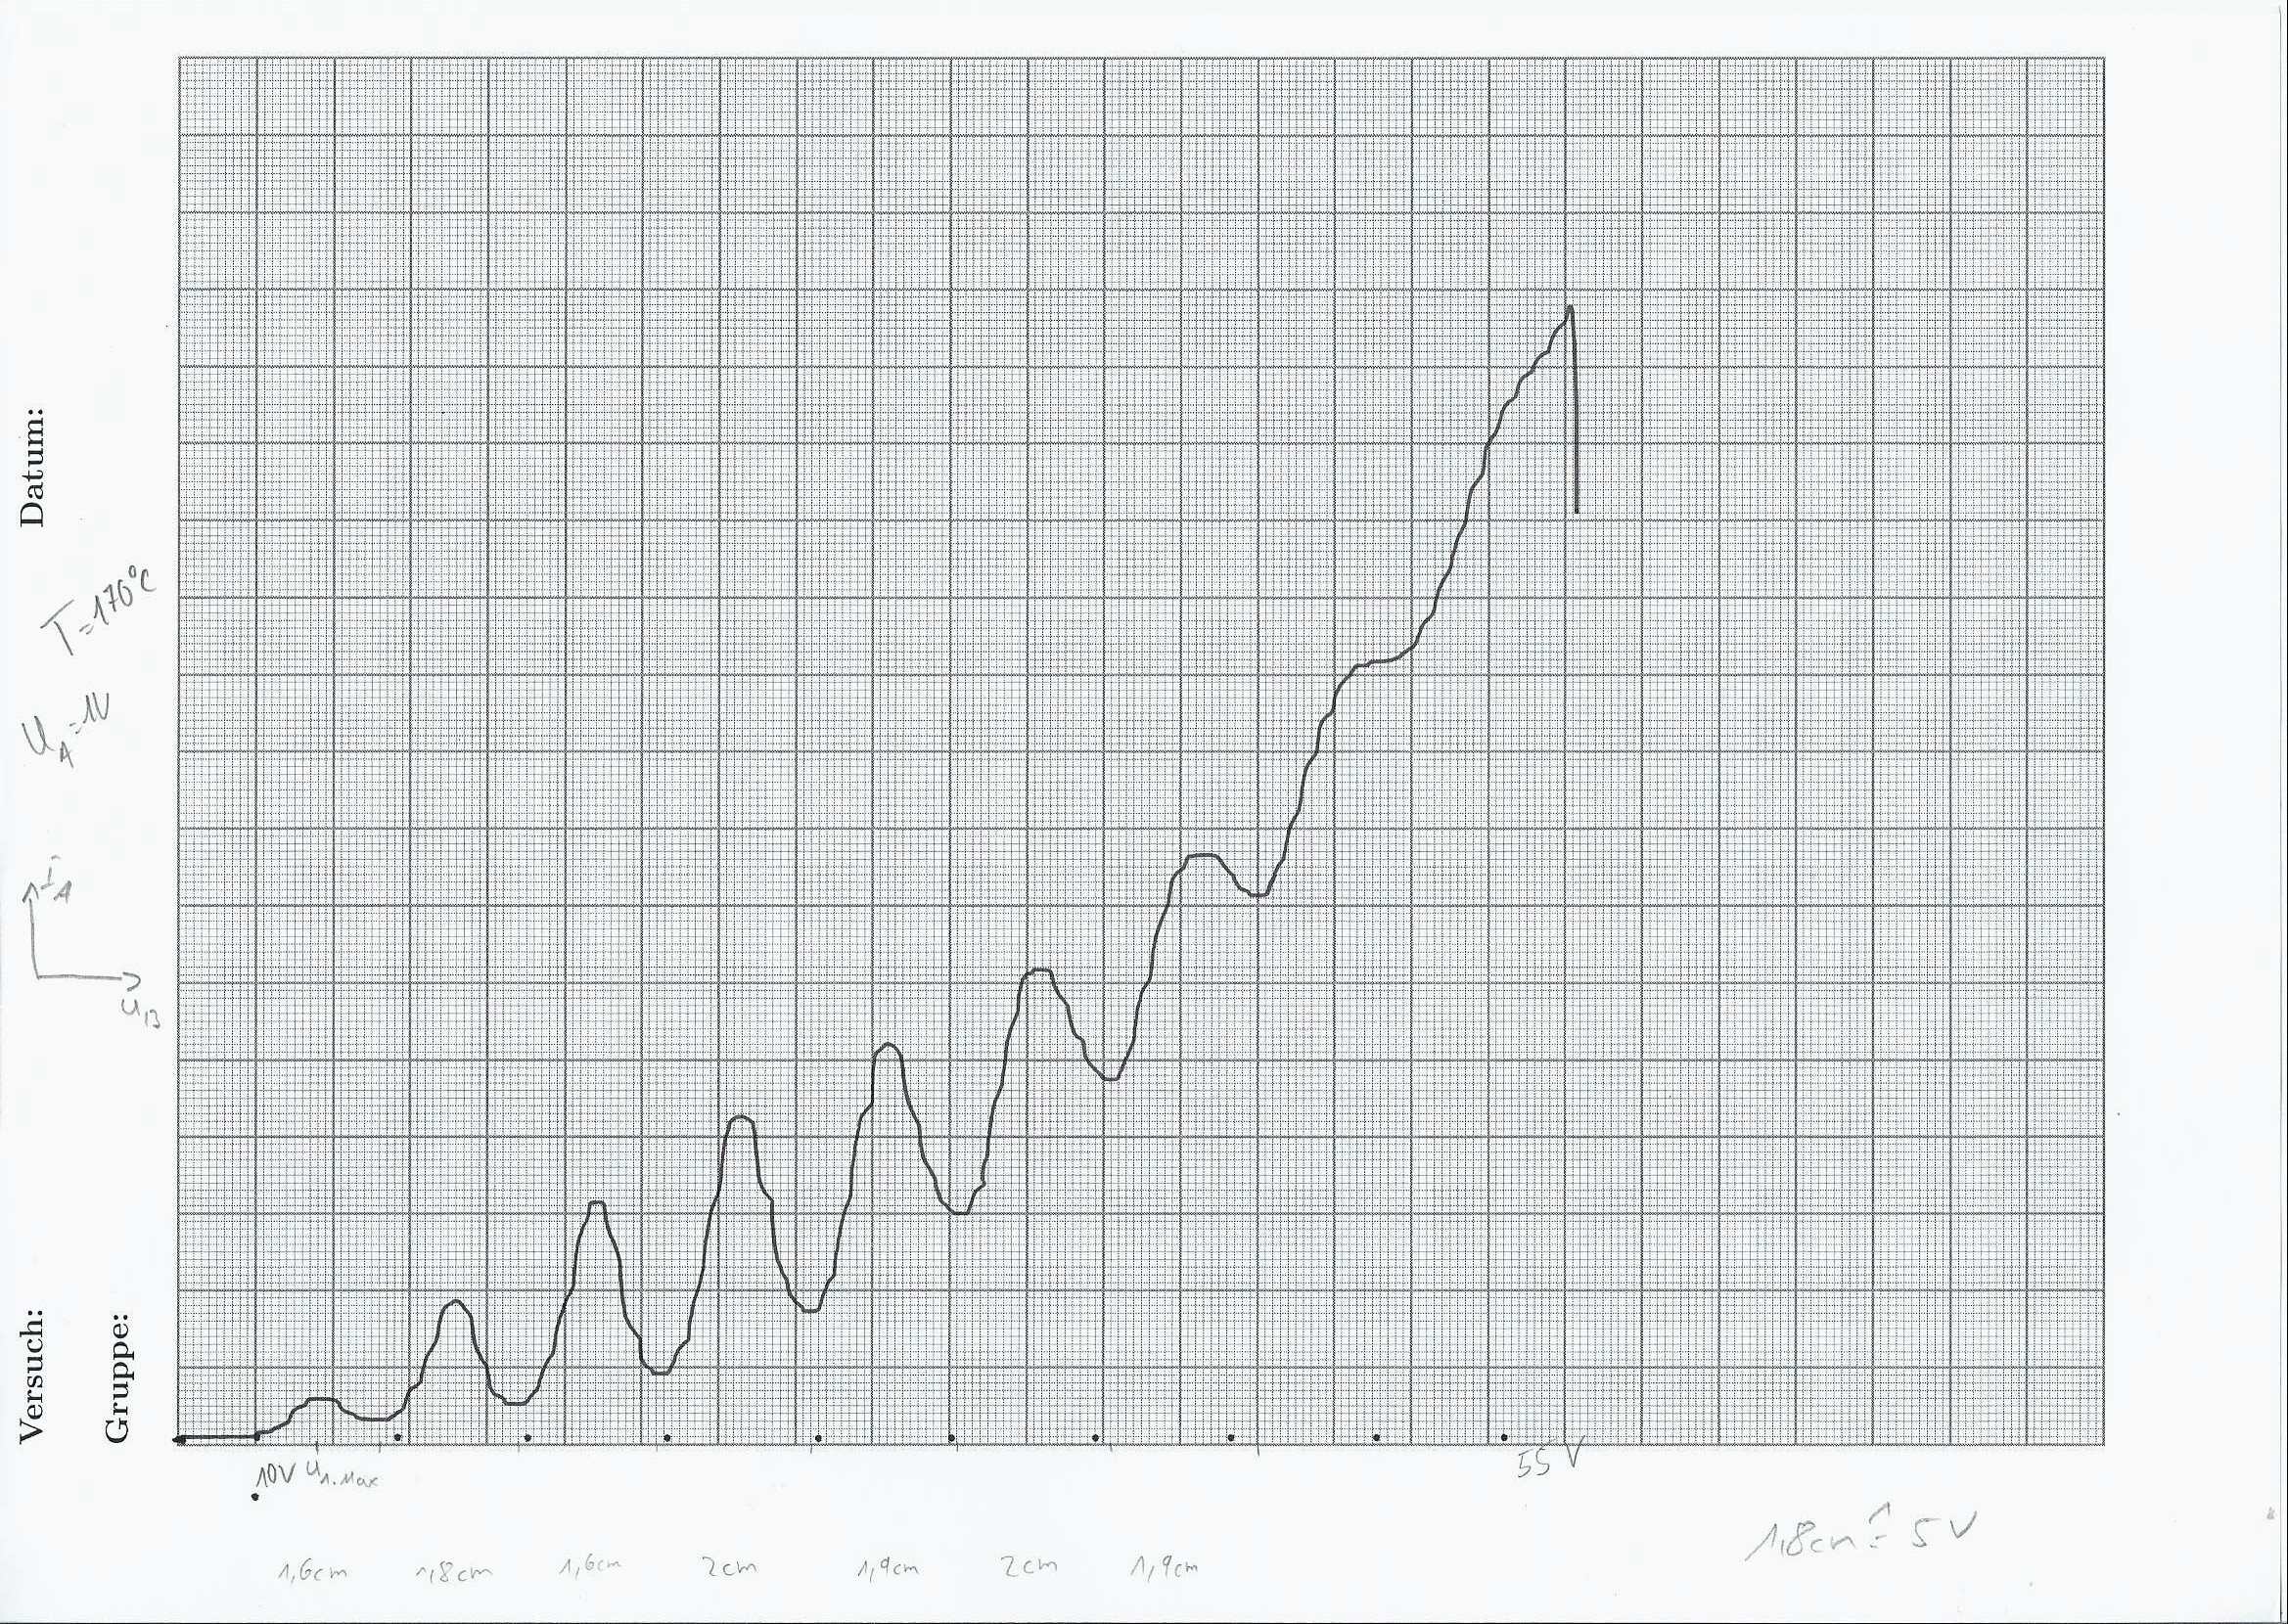
\includegraphics[width=0.8\textwidth]{bilder/kurve.pdf}
  \caption{Idealisierter Zusammenhang zwischen Auffängerstrom und Beschleunigerspannung
  \cite{601}}
  \label{fig:kurve}
\end{figure}
Der Abstand zweier Maxima $U_1$ ist gleich dem ersten Anregungspotential
\begin{equation*}
  U_1:=\frac{1}{e_0}(E_1-E_0)
\end{equation*}
des Quecksilber-Atoms.
